\chapter{Theoretical Background}

\section{Cloud Computing}
Cloud computing refers to the hardware, systems software, and applications delivered as services over the Internet \cite{cloud}. Cloud computing have services from a simple web services to data centers. Hardware for cloud computing can to consist of thousands of individual \emph{computing nodes} with their corresponding networking and storage subsystems, power distribution and conditioning equipment, and extensive cooling systems. Software for cloud computing can to consist of operative system in virtual machines, web applications and web services. 

Cloud computing have three deployment models: \emph{public, private} and \emph{hybrid}, and cloud services models can be grouped three categories:
\begin{itemize}
  \item Infraestructure as a Service(IaaS): providers offer computer power and   storage such as processors, virtual machines, data centers, serves, among others.
  \item Platform as a service(PaaS): providers offer the tools for developing applications such as operative systems, programming languages environments, databases among others.
  \item Software as a Service(SaaS): providers offer access to applications and databases.
\end{itemize}  

Figure \ref{cloud_services} show the stack estructure for cloud services.

\begin{figure}[!h]
\centering
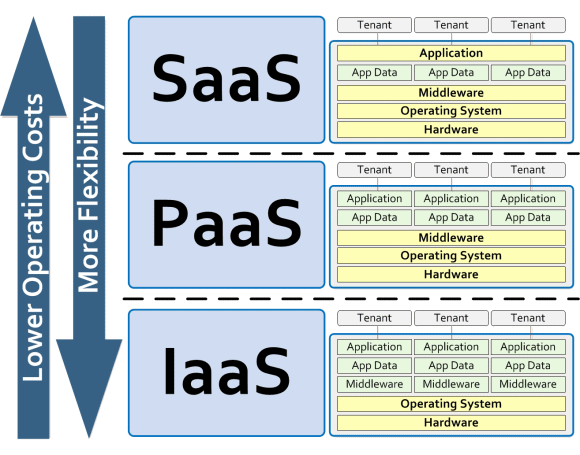
\includegraphics[width=0.5\textwidth]{images/cloud_services}
\caption[Cloud computing service models]{Cloud computing service models 
\textbf{Source:} \url{http://www.ibm.com/developerworks/websphere/techjournal/1206_dejesus/1206_dejesus.html}}
\label{cloud_services}
\end{figure}

\subsection{Virtualisation}

Virtualisation are a important component for cloud computing to decoupled the operative system of the physical infrastructure for adding flexibility. Virtualisation allows rapid deployment, reduce space and energy costs thanks to in a server can be running multiple operative systems. The main aim of virtualisation technologies 
is to hide the physical characteristics of computing resources from the way in which other systems, applications, or end users interact with those resources \cite{virtualization}. Hardware platform, operative system, networks and storage devices can be virtualised. 

\subsubsection{Virtual Machines}
A Virtual Machine(VM) is an instance of the physical machine and gave users the illusion of accessing the physical machine directly \cite{virtualization}. VMs are created and executed in a host machine by Virtual Machine Monitor or Hypervisor. The VMs can run legacy applications requiring an older platform and/or OS and run isolated of the underlying system. Also, it can create a single system image starting from an heterogeneous collection of machines, and can be performed faster job migration within different virtual machines running on the same hardware. These characteristics have led to the use of virtual machines for cloud computing. 

\subsubsection{Network Function Virtualisation}
The Network Function Virtualisation(NFV) involves the implementation of network functions in software that can run on a range of industry standard server hardware, and that can be moved to, or instantiated in, various locations in the network as required, without the need for installation of new equipment \cite{nfv}. European Telecommunications Standards Institute (ETSI) define a NFV framework \cite{nfv_framework} with three main working domains like is showed in figure \ref{nfv_framework}. 


\begin{figure}[!h]
\centering
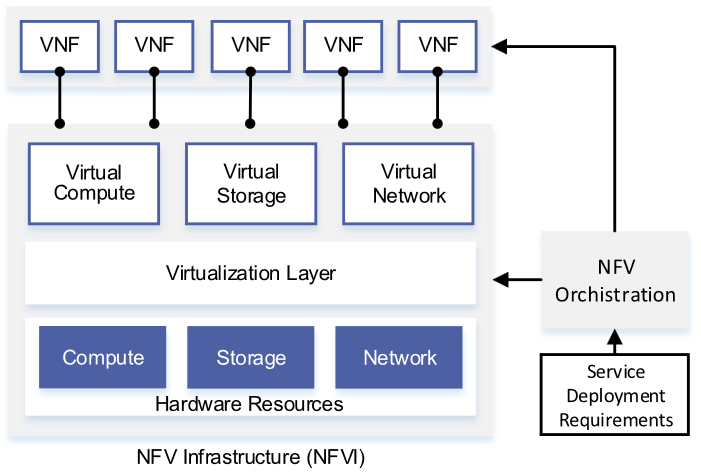
\includegraphics[width=0.5\textwidth]{images/nfv_framework}
\caption[Network Function Virtualisation Framework]{Network Function Virtualisation Framework
\textbf{Source:} Software-Defined Network Function
Virtualisation: A Survey - Figure 1}
\label{nfv_framework}
\end{figure}

The \emph{Virtualised Network Functions} (VNF) are the software implementation of a network function, \emph{NFV Infrastructure} (NFVI) including the diversity of physical resources and \emph{NFV Management and Orchestration} which covers the orchestration and life-cycle management of physical.
and/or software resources 

\subsubsection{Software-defined Network} 
Software-defined Networking (SDN) is a paradigm where a central software program, called a controller, dictates the overall network behavior\cite{sdn}. Basically, it separates vertical integration between the \emph{data plane} (networks control logic) and the \emph{control plane} (routers and switches). A \emph{logically centralized software program}   (or network operative system) implements the logic control of the network, and switches and routers become  simple forwarding devices. The figure \ref{sdn} shows the SDN architecture.

\begin{figure}[!h]
\centering
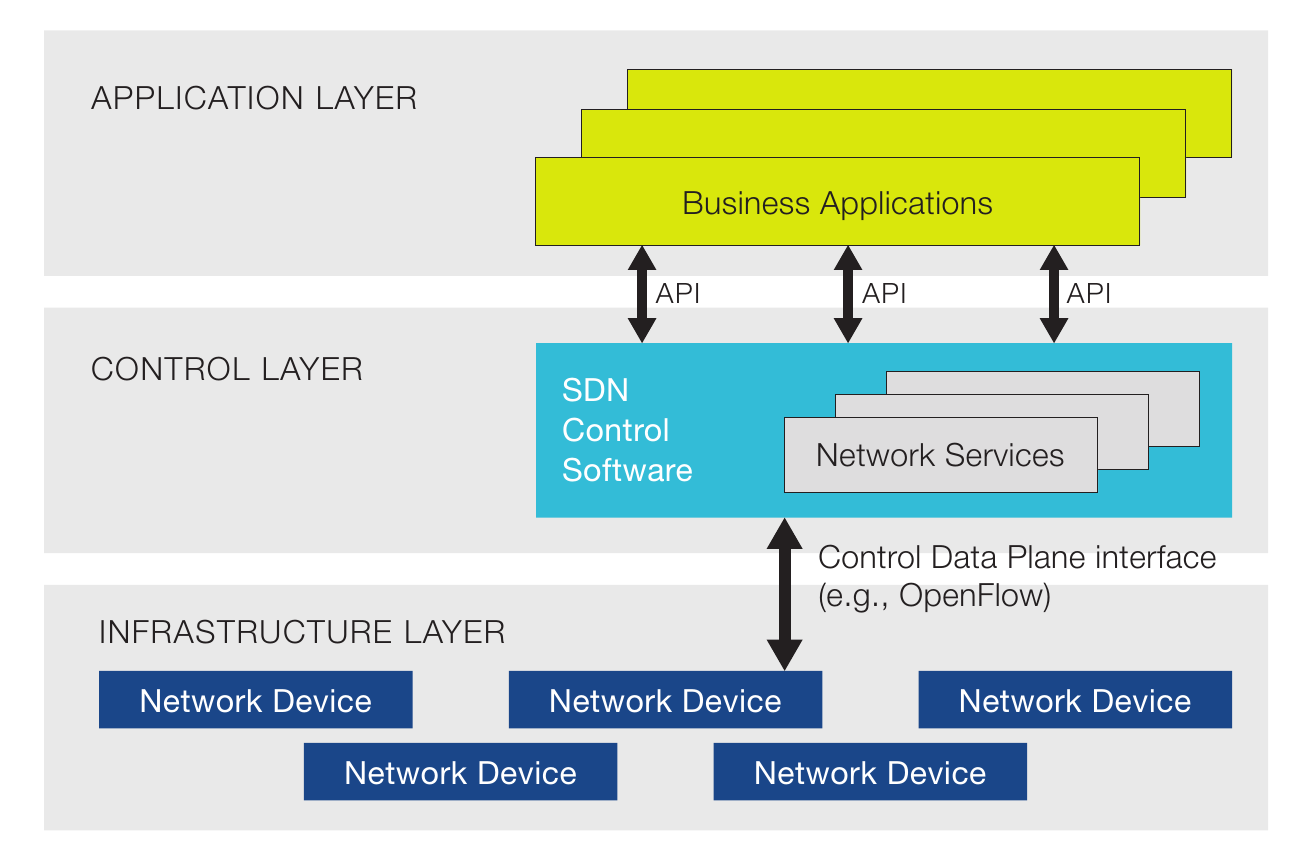
\includegraphics[width=0.5\textwidth]{images/sdn_architecture}
\caption[Software-define Networking]{Software-define Networking
\textbf{Source:} \url{https://www.sdxcentral.com/resources/sdn/inside-sdn-architecture/}}
\label{sdn}
\end{figure}

\section{Fog Computing}
Fog computing, also termed \emph{edge computing}, is considered a an extension of the cloud computing paradigm and it is a proposed paradigm to enable computing directly at the edge of the network \cite{fog}. This paradigm is a highly virtualised platform that provides compute, storage, and networking services without going to the cloud. The devices that are part of the fog computing infrastructure are called \emph{fog nodes} and they provide resources for services at the edge of the network. Fog nodes can be set-top-boxes, access points, routers, switches, base stations and end devices. They are interconnected and and each of them
is linked to the cloud. The figure \ref{fog} shows the fog computing architecture. In this figure can be observed that fog computing between the core and the edge of the network.

\begin{figure}[!h]
\centering
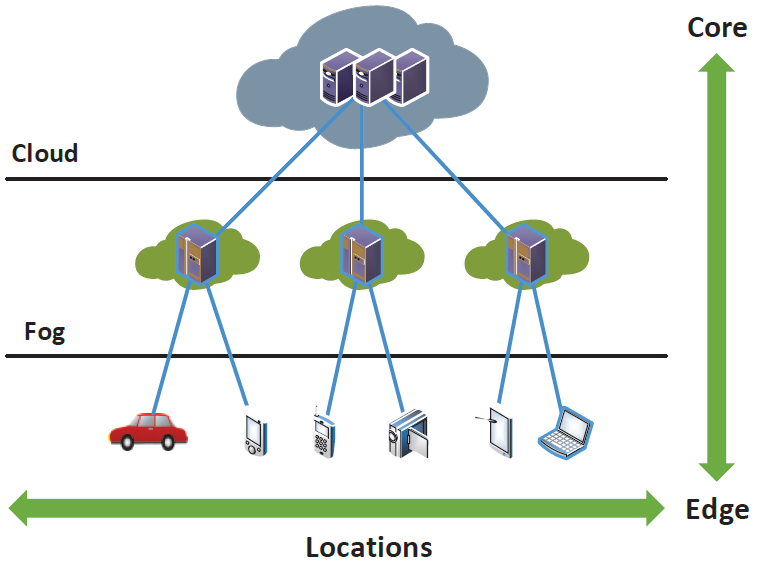
\includegraphics[width=0.5\textwidth]{images/fog}
\caption[Fog Computing Paradigm]{Fog Computing Paradigm
\textbf{Source:} The Fog Computing Paradigm Scenarios and Security Issues - Figure 1}
\label{fog}
\end{figure}

Fog computing includes the same services offered by cloud computing but closer to the end user and so provides low latency, location awareness, and improves quality-of-services (QoS) for streaming and real time applications like video streaming.

\section{Video Coding}





